\documentclass{mimosis}

% get commands and stuff
% Import packages
\usepackage{etoolbox}          % No clue what this does to be honest.

\usepackage[utf8]{inputenc}    % accept both α and \alpha

\usepackage{graphicx, color}   % For making mice coloured text.

\usepackage{scrhack}           % supress warning. No idea why this works.

\usepackage{textcomp,gensymb}  % Extra symbols, like \celsius.

\usepackage{lipsum}            % For making dummy text
\usepackage{blindtext}         % idem dito

\usepackage[stretch=15]{microtype} % prevents many bad hboxes by allowing stretch of letters by 1.5%
\usepackage{mathtools}         % Tools for maths

\usepackage{siunitx}           % To write nice SI units

\usepackage{listings}          % for showing code nicely

\usepackage[%
  colorlinks = true,
  unicode,
]{hyperref}                    % set internal link colors. Will be set to chapter colors in the mainmatter. The values here are just the fallback and I could just have left them out.

\usepackage{url}               % needed to properly show some links in the bibliography.

\usepackage[perpage,symbol*]{footmisc} % For making footnotes nice (and different from regular references to literature)

\usepackage{epigraph}          % for showing quotes at new chapters

\usepackage{tabularx}          % Package for fancy tables

\usepackage{adjustbox}         % package for making tables fit on 1 page

% These two packages are for cycling trough colours depending on the chapter.
% (optional)
\usepackage{pgffor}
\usepackage{pgfmath}
         % Imports all packages you need Mimosis does not contain.
% Bibliography options can get messy, so I gave them their own file

% If you have bibliography line-break problems check https://tex.stackexchange.com/a/442317

\usepackage[
  backend=bibtex,     % If you have biber (you probably do), put 'biber' here.
  citestyle=numeric-comp, % decide for yourself
  sorting=none,
  maxnames=99,        % just put everyones name there, a thesis can be as long as you like anyway
  maxcitenames=99,    % idem dito.
  block = space,      % This will grow and shrink space between elements of the citation (e.g. authors and title), may not look as pretty, but will take care of headache.
  backref=true,
  backrefstyle=three, % I persanally always like backreferences.
  doi=true,           % I love DOIs
  eprint=false,       % typically unneeded if you have doi
  isbn=false,         % do not print isbn or issn numbers, cause no-one uses those.
  defernumbers=true,  % The bibliography and digital resources thing have seperate numbering. Not required if you just have one bibliography.
]{biblatex}

\addbibresource{thesislib.bib} % Import the bibliography file. Generate from Zotero or Mendeley, or write yourself if you hate yourself.

% To only show URLs when no DOI is available, see https://tex.stackexchange.com/a/439818:
\letbibmacro{urlBAK}{url}
\renewbibmacro{url}{\iffieldundef{doi}{\usebibmacro{urlBAK}}{}}

\renewcommand*{\bibfont}{\small} %Make bibliographies have a smaller font to save on printing costs

% Make linebreaks possible for DOIs in bib entries, see:
% https://tex.stackexchange.com/questions/134191/line-breaks-of-long-urls-in-biblatex-bibliography
\setcounter{biburlnumpenalty}{7000}
\setcounter{biburllcpenalty}{7000}
\setcounter{biburlucpenalty}{8000}

% Remove the month field from the bibliography. It does not serve a good
% purpose, I guess. And often, it cannot be used because the journals
% have some crazy issue policies.
\AtEveryBibitem{\clearfield{day}}
\AtEveryCitekey{\clearfield{day}}

\AtEveryBibitem{\clearfield{month}}
\AtEveryCitekey{\clearfield{month}}

% Also clear the visited time, cause that is useless info.
\AtEveryBibitem{
    \clearfield{urlyear}
    \clearfield{urlmonth}
}

% Cite movie and video types as if it is misc (this is default behaviour, but it supresses a warning)
\DeclareBibliographyAlias{movie}{misc}
\DeclareBibliographyAlias{video}{misc}

% You could put a note before the bibliography begins here. This is put after the heading, but before the citations begin. Maybe you have a funny quote or something.
\defbibnote{myprenote}{
    This is an example note, that will appear before the actual bibliograhpy will start.
}

\defbibnote{predigitalmaterialsnote}{
    The following are references to content that can be found online.
} % Imports bibliography settings
%%%%%%%%%%%%%%%%%%%%%%%%%%%%%%%%%%%%%%%%%%%%%%%%%%%%%%%%%%%%%%%%%%%%%%%%
% Fonts
%%%%%%%%%%%%%%%%%%%%%%%%%%%%%%%%%%%%%%%%%%%%%%%%%%%%%%%%%%%%%%%%%%%%%%%%

\ifxetexorluatex
  \setmainfont{Minion Pro}
\else
  \usepackage[lf]{ebgaramond}
  \usepackage[oldstyle,scale=0.7]{sourcecodepro}
  \singlespacing
\fi

\renewcommand{\th}{\textsuperscript{\textup{th}}\xspace}

%%%%%%%%%%%%%%%%%%%%%%%%%%%%%%%%%%%%%%%%%%%%%%%%%%%%%%%%%%%%%%%%%%%%%%%%
% Change page size
%%%%%%%%%%%%%%%%%%%%%%%%%%%%%%%%%%%%%%%%%%%%%%%%%%%%%%%%%%%%%%%%%%%%%%%%
% This is a horrible subject full of jargon, and completely ununderstandable by non-printing experts like myself, but like this it looks nice! Check koma-script docs on CTAN, Chapter 2 for an explenation.
% Basically, these options try to limit the number of charachters on a single line, because if there are ~80+ charachters, it becomes tiring to read. To set the correct margins etc, KOMA needs to know the font size, paper size, etc., so that is why I need to re-run it here.
\KOMAoptions
  {
    paper=170mm:240mm,  % 17x24 cm is Dutch Thesis standard size.
    DIV=calc,           % automatically work out how wide text should be, etc..
    twoside=false,      % a digital copy is of course not two-sided! So set this to 'false' for the digital reading version for the comittee, and turn it to 'true' or 'semi' for the printing copy you need to send to the press. See below for difference between true and semi.
    BCOR = 0mm,         % This is the so-called binding correction, the amount of paper that 'disapears' into the spine of the booklet. It basically offsets your text from the center to account for this. You can probably ignore this value.
  }
\recalctypearea % to apply the options

% If twoside = true, this has the (seemingly) weird effect of getting much larger empty margin space on the outer edges then the inner edges of the paper, but this actually sort of makes sense! Since this will be a booklet, the two inner margins together will actually be the same size as the individual outer margins. If you don't like the way this looks (like me), set this to `semi`, and the margins will look normal.

%%%%%%%%%%%%%%%%%%%%%%%%%%%%%%%%%%%%%%%%%%%%%%%%%%%%%%%%%%%%%%%%%%%%%%%%
% Draft settings
%%%%%%%%%%%%%%%%%%%%%%%%%%%%%%%%%%%%%%%%%%%%%%%%%%%%%%%%%%%%%%%%%%%%%%%%
% Turn these off for the final version!
\KOMAoptions{overfullrule=true}    % Line next to overly long lines (if present)

%%%%%%%%%%%%%%%%%%%%%%%%%%%%%%%%%%%%%%%%%%%%%%%%%%%%%%%%%%%%%%%%%%%%%%%%
% Caption settings
%%%%%%%%%%%%%%%%%%%%%%%%%%%%%%%%%%%%%%%%%%%%%%%%%%%%%%%%%%%%%%%%%%%%%%%%
\KOMAoptions
  {
    captions=nooneline,            % makes 1 line captions behave the same as multiline captions. (I think it is) Very ugly if you don't do this.
  }
\setcapindent{0.5em}               % Change size of indenting in second line of captions

%%%%%%%%%%%%%%%%%%%%%%%%%%%%%%%%%%%%%%%%%%%%%%%%%%%%%%%%%%%%%%%%%%%%%%%%
% Make the distance between float and text smaller
%%%%%%%%%%%%%%%%%%%%%%%%%%%%%%%%%%%%%%%%%%%%%%%%%%%%%%%%%%%%%%%%%%%%%%%%
% makes distance between Figures and text smaller. Wastes less space on your pages with whitespace
\setlength{\textfloatsep}{5pt plus 2pt minus 2pt}

%%%%%%%%%%%%%%%%%%%%%%%%%%%%%%%%%%%%%%%%%%%%%%%%%%%%%%%%%%%%%%%%%%%%%%%%
% Float placements
%%%%%%%%%%%%%%%%%%%%%%%%%%%%%%%%%%%%%%%%%%%%%%%%%%%%%%%%%%%%%%%%%%%%%%%%
% Max number of figures/tables on one page is 1, also, they can take at most `\XXXfraction' of the page, before they are forced onto a page just for the figure.
\renewcommand{\topfraction}{1}
\renewcommand{\bottomfraction}{1}
\renewcommand{\textfraction}{0}
\setcounter{totalnumber}{1}
\setcounter{bottomnumber}{1}
\setcounter{topnumber}{1}

%%%%%%%%%%%%%%%%%%%%%%%%%%%%%%%%%%%%%%%%%%%%%%%%%%%%%%%%%%%%%%%%%%%%%%%%
% Titlepage
%%%%%%%%%%%%%%%%%%%%%%%%%%%%%%%%%%%%%%%%%%%%%%%%%%%%%%%%%%%%%%%%%%%%%%%%
% In printing books, it is normal to include a cover page before the 'real' titlepage, so we do that as well. Settings about that go here.

\renewcommand*{\titlepagestyle}{empty} % No page numbers on this page!

%%%%%%%%%%%%%%%%%%%%%%%%%%%%%%%%%%%%%%%%%%%%%%%%%%%%%%%%%%%%%%%%%%%%%%%%
% Settings for the abstract at the beginning of a chapter
%%%%%%%%%%%%%%%%%%%%%%%%%%%%%%%%%%%%%%%%%%%%%%%%%%%%%%%%%%%%%%%%%%%%%%%%
\newcommand\abstractwidth{0.85} % width of abstract as fraction of pagewidth

%%%%%%%%%%%%%%%%%%%%%%%%%%%%%%%%%%%%%%%%%%%%%%%%%%%%%%%%%%%%%%%%%%%%%%%%
% Epigraph settings (quote boxes)
%%%%%%%%%%%%%%%%%%%%%%%%%%%%%%%%%%%%%%%%%%%%%%%%%%%%%%%%%%%%%%%%%%%%%%%%
\renewcommand{\epigraphflush}{center} % center epigraphs.
\setlength{\epigraphwidth}{6.5cm} % set width of epigraph.

%%%%%%%%%%%%%%%%%%%%%%%%%%%%%%%%%%%%%%%%%%%%%%%%%%%%%%%%%%%%%%%%%%%%%%%%
% Show Bibliography in Content section
%%%%%%%%%%%%%%%%%%%%%%%%%%%%%%%%%%%%%%%%%%%%%%%%%%%%%%%%%%%%%%%%%%%%%%%%
% Removing this will remove bib from the toc completely. It does not actually number the bibliography section, which I think is weird.
\KOMAoptions{bibliography=numbered}
\KOMAoptions{toc=bibliographynumbered}

%%%%%%%%%%%%%%%%%%%%%%%%%%%%%%%%%%%%%%%%%%%%%%%%%%%%%%%%%%%%%%%%%%%%%%%%
% Settings for colouring the number in chapters, (sub-)sections, and 
% captions
%%%%%%%%%%%%%%%%%%%%%%%%%%%%%%%%%%%%%%%%%%%%%%%%%%%%%%%%%%%%%%%%%%%%%%%%
% In this template, every chapter has its own theme color, set that up here
% If you just want 1 consistent color, just repeat the same color a lot of times.

% definition of colours (outside of regular definitions)
% check also here: https://latexcolor.com/
% for instance:
\definecolor{deep-azure}            {RGB}{  10,  50,  94}
\definecolor{bluegray}              {rgb}{0.4, 0.6, 0.8}
\definecolor{palecarmine}           {rgb}{0.69, 0.25, 0.21}
\definecolor{persianplum}           {rgb}{0.44, 0.11, 0.11}
\definecolor{brightmaroon}          {rgb}{0.76, 0.13, 0.28}
\definecolor{darktangerine}         {rgb}{1.0, 0.66, 0.07}
\definecolor{britishracinggreen}    {rgb}{0.0, 0.26, 0.15}
\definecolor{tpyellow}              {HTML}{DDAA33}
\definecolor{tpred}                 {HTML}{BB5566}
\definecolor{tpdblue}               {HTML}{004488} 
\definecolor{tpgreen}               {HTML}{38993E}

% define the colours to cycle trough (see https://tex.stackexchange.com/questions/99429/chapter-colorized-in-different-colors)
% there is no "chapter 0", so ther is a dummy at index=0.
% This array needs to be a bit longer than the actual number of chapters. So fill it out with dummies.

\def\colourarray{{"deep-azure", "deep-azure", "bluegray", "palecarmine", "persianplum", "brightmaroon", "darktangerine", "britishracinggreen", "tpyellow", "tpred", "tpdblue", "tpgreen"}} 


% Now actually set the colours below:
% Colour for chapter numbers
\renewcommand*{\chapterformat}{%
  \fontsize{50}{55}\selectfont\pgfmathparse{\colourarray[\thechapter]}\textcolor{\pgfmathresult}{\thechapter}\autodot\enskip
}
% how is this built up?
% \fontsize speaks for itself, \selectfont too. 
% \pgfmathparse{\colourarray[\thechapter]} takes the index in the array with the chapter number and looks what the colour is
% \textcolor{\pgfmathresult} takes the result and actually colours the chapter number
% The other (sub-)sections etc. below are built in the same way, based on the chapter number so sections have the same color as chapters.

% Colour for section numbers
\renewcommand*{\sectionformat}{%
\pgfmathparse{\colourarray[\thechapter]}\textcolor{\pgfmathresult}{\thesection}\autodot\enskip%
}

% Colour for subsection numbers
\renewcommand*{\subsectionformat}{%
\pgfmathparse{\colourarray[\thechapter]}\textcolor{\pgfmathresult}{\thesubsection}\autodot\enskip%
}

% Colour for subsubsection numbers
\renewcommand*{\subsubsectionformat}{%
\pgfmathparse{\colourarray[\thechapter]}\textcolor{\pgfmathresult}{\thesubsubsection}\autodot\enskip%
}

% Colour for Figure/table numbers:
\setkomafont{captionlabel}{ \pgfmathparse{\colourarray[\thechapter]} \color{ \pgfmathresult } \small}
 % For using mimosis with my own settings
%To make simple comments in the text
\newcommand{\com}[1]{\textcolor{red}{#1}}
%To define the vector command (which will just make math FAT)
\renewcommand{\vec}[1]{\mathbf{#1}}
%To make any chemical formulas look like chemical formulas
\newcommand*\chem[1]{\ensuremath{\mathrm{#1}}}
% to make Molar a usable unit
\DeclareSIUnit\Molar{\textsc{M}}
% To make some chemicals properly hyphenated
% \hyphenation{
%     er-go-no-mic,% example
%     tri-me-thoxy-silyl,
%     me-tha-cry-late,
%     lu-ti-dine,
% }

% I really don't care about hyphenation in the bibliography, and some names are just not hyphenated, super annoying. So force the matter here.
\hyphenation{S-c-i-o-r-t-i-n-o}
\hyphenation{S-c-h-w-a-r-t-z} % User defined commands

% I prefer to put images in a folder for the chapter itsself. You can also put all images in a single dedicated folder, in that case, you can set that here:
% \graphicspath{{./images/}}

% Set up your cover page:
\title{An example thesis}
\subtitle{A clever joke as subtitle always works well}
\author{P.J.M. Swinkels}
\date{}

% Set pdf metadata:
\hypersetup{%
    pdfauthor={Piet J.M. Swinkels},
    pdftitle={An example thesis: A clever joke as subtitle always works well},
    pdfsubject={Soft Matter Physics},   % Or whatever the subject of your thesis is
    pdfkeywords={Soft matter; Self-assembly; Colloids; Patchy particles; Critical Casimir effect},
}

% If you don't want to regenerate the entire thesis every time you make changes, you can turn on and off what is regenerated in this list:
\includeonly{
    Sections/Preface/officialtitlepage,
    Sections/Preface/comitteepage,
    Sections/Preface/colophon,
	Sections/Preface/niceinterlude,
    Sections/Chapter1/chapter1,
    Sections/Chapter2/chapter2,
    Sections/Chapter3/chapter3,
    Sections/Chapter4/chapter4,
    Sections/Chapter5/chapter5,
    Sections/Chapter6/chapter6,
    Sections/Chapter7/chapter7,
    Sections/Chapter8/chapter8,
    Sections/Postface/acknowledgements,
    Sections/Postface/closingstatement,
    Sections/Postface/listofpublications,
}

\begin{document}
    \hypersetup{
        citecolor  = black,
        linkcolor  = black,
        urlcolor   = black,
    }                                            % Links and refs should just be black outside of the chapters with an accent colour.
    \maketitle                                   % This is the coverpage, most books have a sort of pre-titlepage immediatly after the outside cover, with just title and author.
    \cleardoubleevenemptypage                    % titlepage should start on the right-hand side. See Readme for more.
    \pagestyle{empty}                            % No page numbers on title page!
    % This is the mandatory, pedel-approved title page.
% Text CANNOT be changed!
% Thanks to https://github.com/mathren/API_thesis_template/blob/master/content/titlepage.tex for a simple LATEX template for these pages

%---------------------------------------------------------------------------
%	COVER PAGE
%---------------------------------------------------------------------------

% \thispagestyle{empty} % No page numbering here!

\begin{minipage}[c][190mm][c]{118mm} %% Full center
  % \begin{minipage}[c][190mm][c]{124mm}  %% 6mm offset from center to right
    % For the print edition I choose to offset the page to compensate for the
    % binding back. This gives the illusion that the title page is centered.
    % For the digital edition I use the true center. 
  \makeatletter
  \begin{center}
      %% Leading whitespace
      \vspace*{1.2cm}
  
      %% Thesis title
      { \huge Colloidal Architectures }\\
      \vspace*{0.2cm}
      { \Large Atom-like Assembly of Patchy Particles }\\ % textsc can be used to makes captioned font for subtitle, but I think its not so nice here.
      [2.7cm]
  
      %% Thesis type
      \textsc{\Large ACADEMISCH PROEFSCHRIFT}\\[1.2cm]
          
      %% Auxiliary details
      \linespread{1.2}
      { \normalsize \textrm{
          ter verkrijging van de graad van doctor \\
          aan de Universiteit van Amsterdam \\
          op gezag van de Rector Magnificus \\
          prof.~dr.~K.~I.~J.~Maex \\
          en overstaan van een door het College voor Promoties ingestelde \\
          commissie, in het openbaar te verdedigen in de Agnietenkapel \\
          op vrijdag 8 juli 2022, te 10.00 uur \\ 
          \vspace{0.9cm}
          door \\[0.3cm]
          \vspace{0.9cm}
          Petrus Johannes Maria Swinkels\\[0.3cm]
          geboren te Tilburg \\[0.3cm]  
      } }
  
  \end{center}
  \makeatother

\end{minipage}
%% Clear out the remaining page
\clearpage % Copied from official pdf
    
    %%%%%%%%%%%%%%%%%%%%%%%
    % The frontmatter starts here. Don't use '\frontmatter' directly, because it will cause an empty page in twopage mode. I could also have redifined \frontmatter, but that would be hard.
    \pagestyle{plain}                            % page numbers for frontmatter (but no header)
    %%%%%%%%%%%%%%%%%%%%%%%

    % This is the mandatory, pedel-approved comittee page.
% Text CANNOT be changed, except for the funding info at the end.
% Thanks to https://github.com/mathren/API_thesis_template/blob/master/content/titlepage.tex for a simple LATEX template for these pages

%-----------------------------------------------------------------------------
%	DOCTORAL BOARD
%-----------------------------------------------------------------------------
% Custom header type
{\small \textit{Promotiecommissie:}} \\[0.2cm]

% List boardmembers
{ \footnotesize % if your boardmembers have shorter names, you can make the font size larger. If they have long names, it's probably best to enforce a line break.
\begin{tabular}{@{}lll}
\textit{Promotor:}      & prof.~dr.~P. Schall    & Universiteit van Amsterdam\\
~                       & ~                      & ~                         \\
\textit{Copromotor:}    & dr.~C.J.M. Coulais     & Universiteit van Amsterdam\\
~                       & ~                      & ~                         \\
\textit{Overige leden:} & dr.~M. Jalaal          & Universiteit van Amsterdam\\
                        & prof.~dr.~S. Woutersen & Universiteit van Amsterdam\\
                        & prof.~dr.~P.G. Bolhuis & Universiteit van Amsterdam\\
                        & prof.~dr.~ir.~J. van der Gucht & Wageningen University~\&~Research \\
                        & dr.~D. Chakrabarti    & University of Birmingham \\
\end{tabular} 
}

\vspace*{0.8cm}
% Note faculty

{\small Faculteit der Natuurwetenschappen, Wiskunde en Informatica}

% Funding footnote
\vspace*{\fill}

\begin{figure}[!h]
    
\includegraphics[width=1.0\textwidth]{Sections/Preface/logos/full-logo.pdf}
\end{figure}

% Report financial backing of the research (see article 15.5 & 29.6)
% Can also be in English.
\begin{otherlanguage}{dutch}
{\small \noindent Het hier beschreven onderzoek is uitgevoerd binnen de groep van prof.~dr.~Peter~Schall aan het Institute of Physics van de Universiteit van Amsterdam (gevestigd te Science Park 904, 1098 XH, Amsterdam). Het onderzoek is gefinancieerd met steun van de Nederlandse Organisatie voor Wetenschappelijk Onderzoek (NWO), via een persoonlijke toelage (VICI) toegewezen aan prof.~dr.~Peter Schall.} \vspace{0.5em}
\end{otherlanguage}
\clearpage      % Copied from official pdf + funding info.
    % This page contains the ISBN number, cover design credits, copyright information, and probably your email. Maybe also a linkt to the online version of this thesis at a repositoru (like UVA DARE).
% Only needs to be present in the printing version of the thesis.

\vspace*{\fill}

\textbf{ISBN: 123456-7891-798}

\vspace*{0.3cm}

Cover design by Pieter Post \& Petronella Paaltjes

\vspace*{0.3cm}

Copyright © Piet J.M. Swinkels, 2022. All rights reserved.

\vspace*{1.2cm}

A digital copy of this thesis can be obtained via \texttt{\href{https://www.dare.uva.nl/}{dare.uva.nl}}

\vspace*{0.3cm}

The author can be reached at: \texttt{\href{mailto:example@email.com}{example@email.com}}

\vspace*{1.2cm}          % ISBN, etc.
    % This page comes between the official comitteepages and the Content, where the real thesis starts. It cam ne anything you want, a real preface, or just a nice quote like below. It is not required in any way.

\null\vfill\null
\hfill\parbox{110mm}{
  \raggedleft
    \emph{It's still magic, even if you know how it's done.}\\[5pt]
  - Terry Pratchett, A Hat Full of Sky
}
\null\vfill\null     % A quote, or some nice personal words. Not required.
    \setcounter{tocdepth}{\sectiontocdepth}      % select what to show in toc (only sections, not subsections)
    \tableofcontents                             % currently, the toc starts at the left page (in twopage mode), so the entire content can be seen without  flipping through the booklet. You can change that if you feel like it by including '\cleardoubleevenemptypage'

    %%%%%%%%%%%%%%%%%%%%%%%
    % The mainmatter starts here. Again, I don't use \mainmatter directly.
    % \mainmatter
    \pagestyle{headings}                         % page numbers and headers for the remainder of the thesis.
    \KOMAoptions{open=right}                      % Chapters start on the right-hand side in the booklet. 
    
    % But, to leave room for images, start left, leave an empty page/include an image, then start the chapter.
    %%%%%%%%%%%%%%%%%%%%%%%

    %%%%%%%%%%%%%%%%%%%%%%%%%%%%%%%%%%%%%%%%%%%%%%%%%%%%%%%%%%%%%%%%%%%%%%%%
\cleardoubleevenemptypage
\chapter{Introduction}
\label{ch:intro}
%%%%%%%%%%%%%%%%%%%%%%%%%%%%%%%%%%%%%%%%%%%%%%%%%%%%%%%%%%%%%%%%%%%%%%%%
\pgfmathsetmacro\chapclr{\colourarray[1]} % set the number to the chapter number. Yes, by hand. Don't ask me why.
\hypersetup{
  citecolor  = \chapclr,
  linkcolor  = \chapclr,
  urlcolor   = \chapclr,
}

\epigraph{
  A quasi-deep quote, with minimal relevance to the chapter.
  }{
    \textit{Piet J.M. Swinkels}
}

% The intro probably does not need an abstract:
% \begin{center}
%   \begin{minipage}{\abstractwidth\textwidth}
%     \begin{small}
%       Does the intro really need a short abstract?
%     \end{small}
%   \end{minipage}
%   \vspace{0.5cm}
% \end{center}
\clearpage
%%%%%%%%%%%%%%%%%%%%%%%%%%%%%%%%%%%%%%%%%%%%%%%%%%%%%%%%%%%%%%%%%%%%%%%%%%
\section{The first steps}
You know what are some really great papers? These: \cite{gabryelczykHydrogenBondGuidance2019,heesSelfassemblyOppositelyCharged2019,swinkelsRevealingPseudorotationRingopening2021}! Also, if I want to refer to an online video~\cite{ExampleVideo}, I can do that as well. By default, it will end up in a separate bibliography page! Neat! Look at Figure \ref{fig:ch1-dog}b! It is beautiful! 

\subsection{Continue with blind text}

\blindtext[2]
\subsection{Blahblah}
\blindtext[3]
Look at Figure \ref{fig:ch1-dog}b! It is beautiful! 

\begin{figure}
  \centering
  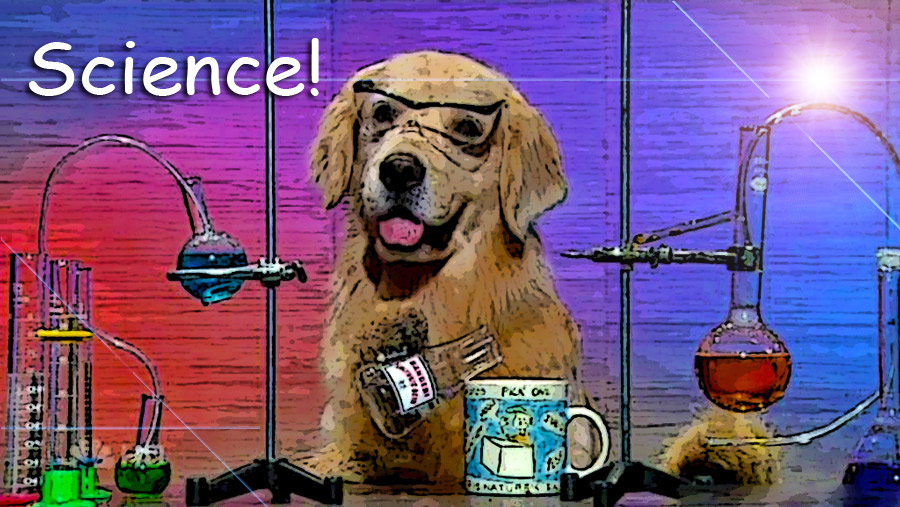
\includegraphics[width=1.0\linewidth]{Sections/Chapter1/Figures/dogs_do_science2.jpg}
  \caption{
    \textcolor{\chapclr}{Pure beauty.}
    I did something and I don't know how, and now I am writing that down somehow. Do you notice how the Figure caption is smaller than the main text, and that there is a small indentation on the left? You can change that! Also, the distance between this text and the main text can be controlled!
    }
  \label{fig:ch1-dog}
\end{figure}

\section{The second step}
\blindtext[1]
\subsection{More questions}
\blindtext[5]

         % This is the intro
    %%%%%%%%%%%%%%%%%%%%%%%%%%%%%%%%%%%%%%%%%%%%%%%%%%%%%%%%%%%%%%%%%%%%%%%%
\cleardoubleevenemptypage
\chapter{Concepts and Methods}
\label{ch:methods}
%%%%%%%%%%%%%%%%%%%%%%%%%%%%%%%%%%%%%%%%%%%%%%%%%%%%%%%%%%%%%%%%%%%%%%%%
\pgfmathsetmacro\chapclr{\colourarray[2]}
\hypersetup{
  citecolor  = \chapclr,
  linkcolor  = \chapclr,
  urlcolor   = \chapclr,
}

\epigraph{
  When you got right down to it, humans were still just curious monkeys. They still had to poke everything they found with a stick to see what it did.
}{
  \textit{James S.A. Correy} \\ Leviathan Wakes
}

\begin{center}
  \begin{minipage}{\abstractwidth\textwidth}
    \begin{small}
      \lipsum[1]
    \end{small}
  \end{minipage}
  \vspace{0.5cm}
\end{center}

\clearpage
%%%%%%%%%%%%%%%%%%%%%%%%%%%%%%%%%%%%%%%%%%%%%%%%%%%%%%%%%%%%%%%%%%%%%%%%%%

\section{First this}
Think back about Chapter \ref{ch:intro}! That was an interesting chapter right? Well, this one will be more interesting!

\blindtext[1]
\subsection{Blahblah}
\blindtext[2]
\section{The second step}
\blindtext[1]
\subsection{More questions}
\blindtext[2]

         % this is the methods section

    % The following chapters are typically based on papers, insert as many as you want:
    %%%%%%%%%%%%%%%%%%%%%%%%%%%%%%%%%%%%%%%%%%%%%%%%%%%%%%%%%%%%%%%%%%%%%%%%
\cleardoubleevenemptypage
\chapter{The first scientific chapter}
\label{ch:pfff}
%%%%%%%%%%%%%%%%%%%%%%%%%%%%%%%%%%%%%%%%%%%%%%%%%%%%%%%%%%%%%%%%%%%%%%%%
\pgfmathsetmacro\chapclr{\colourarray[3]}
\hypersetup{
citecolor  = \chapclr,
linkcolor  = \chapclr,
urlcolor   = \chapclr,
}

\epigraph{
  A quasi-deep quote, with minimal relevance to the chapter.
  }{
    \textit{Piet J.M. Swinkels}
}

\begin{center}
    \begin{minipage}{\abstractwidth\textwidth}
      \begin{small}
        \blindtext[1]
      \end{small}
    \end{minipage}
    \vspace{0.5cm}
\end{center}

\clearpage
%%%%%%%%%%%%%%%%%%%%%%%%%%%%%%%%%%%%%%%%%%%%%%%%%%%%%%%%%%%%%

\section{Introduction}
\blindtext[2]
\section{Results}
\blindtext[1]
\blindmathpaper
\begin{figure}
  \centering
  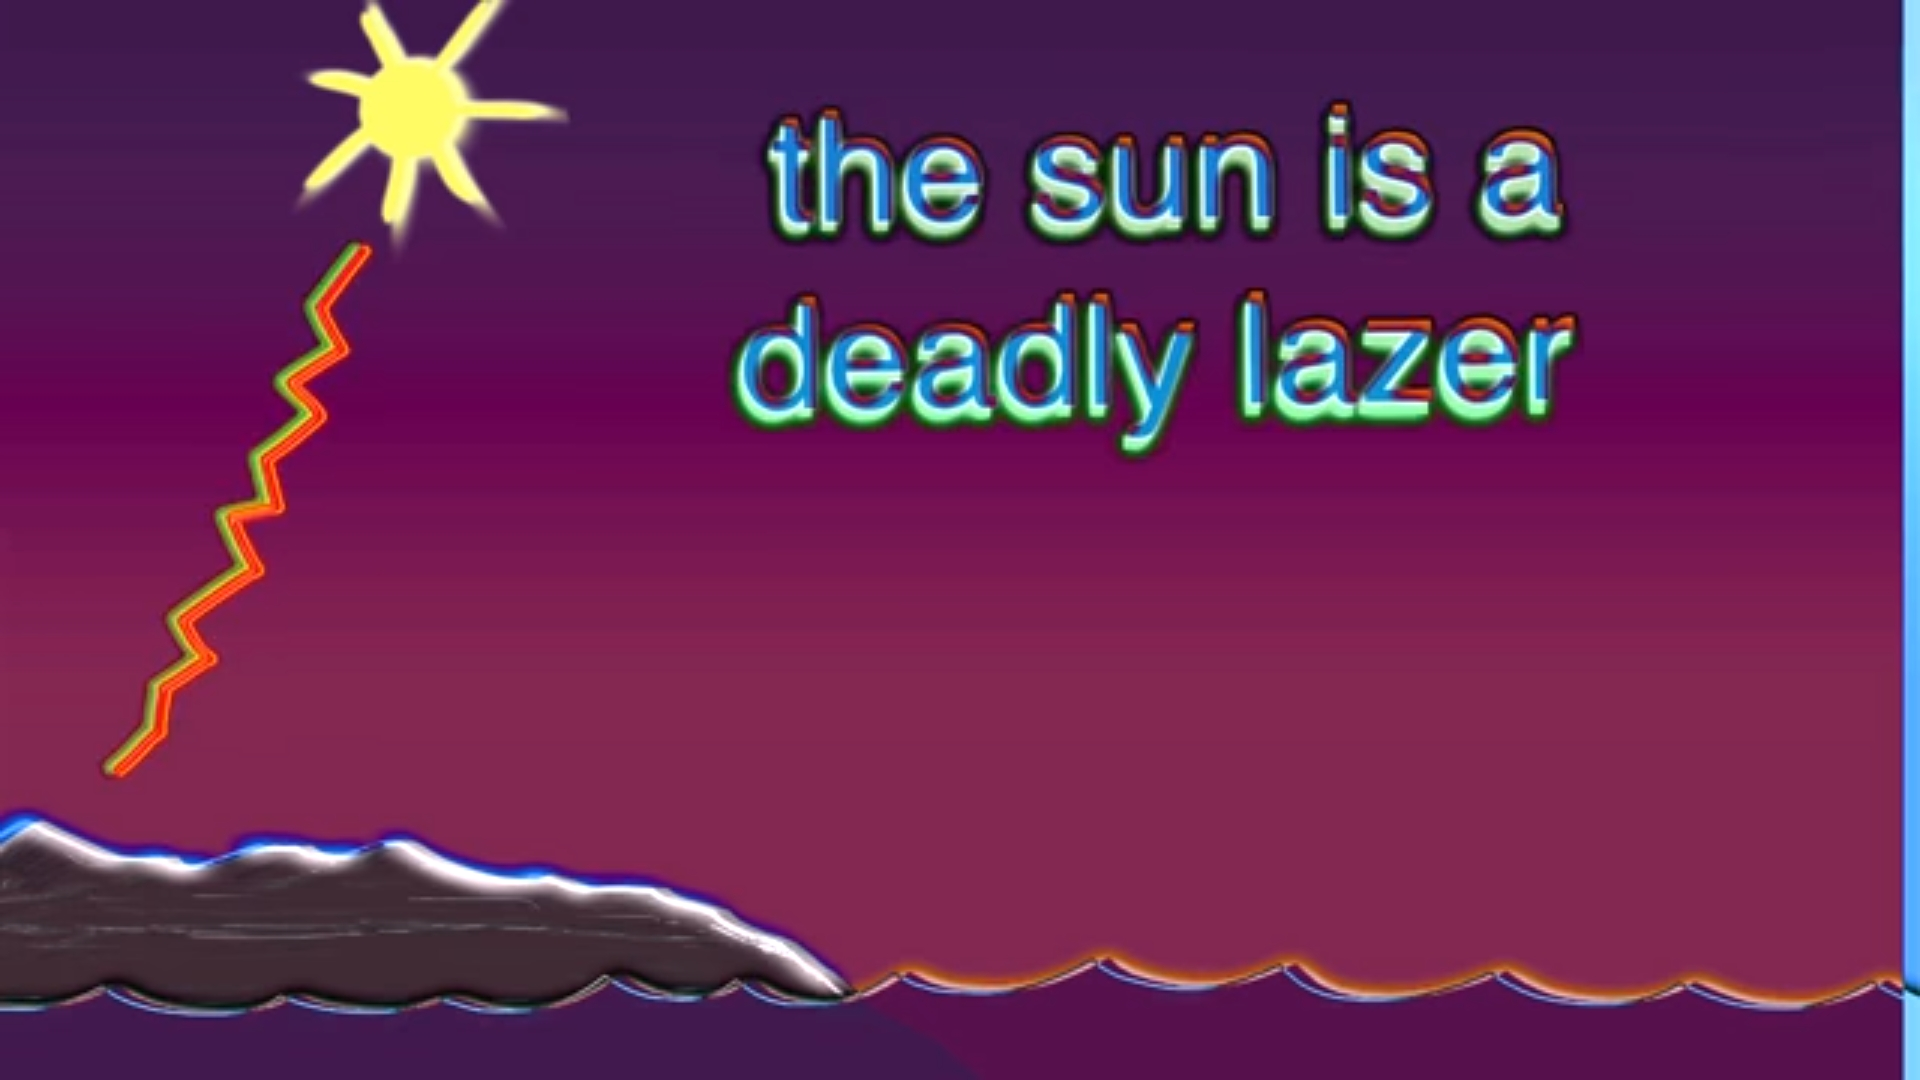
\includegraphics[width=1.0\linewidth]{Sections/Chapter3/Figures/laser.jpg}
  \caption{
    \textcolor{\chapclr}{Pewpewpew.}
    Cool stuff.
    }
  \label{fig:ch3-laser}
\end{figure}
\blindtext[1]
\section{Discussion}
\blindtext[2]

\clearpage

\section{Appendix}

\subsection{Sample preparation and history}

\blindtext[2]

\subsubsection{Math time!}

\blindtext[2]

The angular dependence of the interaction strength is captured by the switching function S which is a smoothly decaying function from 1 to 0 as shown in Figures \ref{fig:ch1-dog}\&\ref{fig:ch3-laser} on the right. We use the switching function

\begin{align}
  &S'(\Theta_i)=
  \begin{cases}
    \frac{1}{2} \left[ 1-\cos \left( \frac{\pi(\cos\Theta_i -\cos\Theta_\mathrm{p})}{1-\cos\Theta_\mathrm{p}} \right) \right]  &  \cos\Theta_i\geq \cos\Theta_\mathrm{p} \\
    0& \cos\Theta_i<\cos\Theta_\mathrm{p}
  \end{cases} \label{eq:ch3-switchfunction}
\end{align}
where $\Theta_\mathrm{p}$ is the patch arc-angle and $\cos\Theta_i=\vec{r_{ij}}\cdot\vec{p}_i/ |\vec{r}_{ij}\cdot\vec{p}_i|$ is the angle between the patch vector $\vec{p}_i$ and the interparticle vector $\vec{r}_{ij}$. 
    %%%%%%%%%%%%%%%%%%%%%%%%%%%%%%%%%%%%%%%%%%%%%%%%%%%%%%%%%%%%%%%%%%%%%%%%
\cleardoubleevenemptypage
\chapter{Another scientific chapter}
\label{ch:anothe-name}
%%%%%%%%%%%%%%%%%%%%%%%%%%%%%%%%%%%%%%%%%%%%%%%%%%%%%%%%%%%%%%%%%%%%%%%%
\pgfmathsetmacro\chapclr{\colourarray[4]}
\hypersetup{
  citecolor  = \chapclr,
  linkcolor  = \chapclr,
  urlcolor   = \chapclr,
}

\epigraph{
  But I am very poorly today and very stupid and hate everybody and everything
}{
  \textit{Charles Darwin}
}

\begin{center}
  \begin{minipage}{\abstractwidth\textwidth}
    \begin{small}
      \lipsum[1]
    \end{small}
  \end{minipage}
  \vspace{0.5cm}
\end{center}

\clearpage
%%%%%%%%%%%%%%%%%%%%%%%%%%%%%%%%%%%%%%%%%%%%%%%%%%%%%%%%%%%%%

\section{Introduction}
Remember the math in the previous chapter? It was eq. \ref{eq:ch3-switchfunction}!

\blindtext[1]

\section{Methods}
\blindtext[1]
\blindenumerate
\blindtext[1]

\section{Results and Discussion}
\blindtext[3]


\section{Conclusion}
\lipsum[2] 
    %%%%%%%%%%%%%%%%%%%%%%%%%%%%%%%%%%%%%%%%%%%%%%%%%%%%%%%%%%%%%%%%%%%%%%%%
\cleardoubleevenemptypage
\chapter{I should have made fewer example chapters}
\label{ch:name}
%%%%%%%%%%%%%%%%%%%%%%%%%%%%%%%%%%%%%%%%%%%%%%%%%%%%%%%%%%%%%%%%%%%%%%%%
\pgfmathsetmacro\chapclr{\colourarray[5]}
\hypersetup{
  citecolor  = \chapclr,
  linkcolor  = \chapclr,
  urlcolor   = \chapclr,
}

\epigraph{
  Memento mori!
}{
  
}

\begin{center}
  \begin{minipage}{\abstractwidth\textwidth}
    \begin{small}
      \lipsum[1]
      \end{small}
  \end{minipage}
  \vspace{0.5cm}
\end{center}

\clearpage
%%%%%%%%%%%%%%%%%%%%%%%%%%%%%%%%%%%%%%%%%%%%%%%%%%%%%%%%%%%%%%%%%%%

\section{Introduction}

\blindtext[2]

\section{Methods}
\blindtext[1]
\blindmathtrue
\blindtext[1]

\section{Results and Discussion}
\blindtext[3]


\section{Conclusion}
\lipsum[1-2]

\clearpage
\section{Appendix}

\subsection{Appendix 1}

\blindtext[1]

\subsection{Appendix 2}

\blindtext[1]

    %%%%%%%%%%%%%%%%%%%%%%%%%%%%%%%%%%%%%%%%%%%%%%%%%%%%%%%%%%%%%%%%%%%%%%%%
\cleardoubleevenemptypage
\chapter{Almost there!}
\label{ch:ch6}
%%%%%%%%%%%%%%%%%%%%%%%%%%%%%%%%%%%%%%%%%%%%%%%%%%%%%%%%%%%%%%%%%%%%%%%%
\pgfmathsetmacro\chapclr{\colourarray[6]}
\hypersetup{
  citecolor  = \chapclr,
  linkcolor  = \chapclr,
  urlcolor   = \chapclr,
}

\epigraph{
  Pupupupupupupupokerface
}{
  \textit{L. Gaga}
}

\begin{center}
  \begin{minipage}{\abstractwidth\textwidth}
    \begin{small}
    This is the last scientific chapter, and probably the worst chapter in your thesis. It is \emph{not} ready for publication, but you really wanted to include it in your thesis, and you just hope the committee will give up reading before they reach this point. 
    \end{small}
  \end{minipage}
  \vspace{0.5cm}
\end{center}

\clearpage
%%%%%%%%%%%%%%%%%%%%%%%%%%%%%%%%%%%%%%%%%%%%%%%%%%%%%%%%%%%%%%%%%%%

\blindtext[2]

\section{Methods}
\blindtext[1]
\blindmathfalse
\blindtext[1]

\section{Results and Discussion}
\blindtext[3]


\section{Conclusion}
\lipsum[1-2]
    
    % Note that a summary is REQUIRED for the reading version of your thesis (the version you send to your comittee). I give it it's own chapter (it is really part of the thesis after all), but some people prefer it to be in the postface, with the acknowledgements and such. You can decide for yourself.
%%%%%%%%%%%%%%%%%%%%%%%%%%%%%%%%%%%%%%%%%%%%%%%%%%%%%%%%%%%%%%%%%%%%%%%%
\cleardoubleevenemptypage
\chapter{Summary}
\label{ch:summary}

\pgfmathsetmacro\chapclr{\colourarray[7]}
\hypersetup{
citecolor  = \chapclr,
linkcolor  = \chapclr,
urlcolor   = \chapclr,
}

\epigraph{
  All good things must come to an end.
}{
  
}
%%%%%%%%%%%%%%%%%%%%%%%%%%%%%%%%%%%%%%%%%%%%%%%%%%%%%%%%%%%%%%%%%%%%%%%%
\lipsum[1-6]         % This is the summary (english)
    % This section is meant for a laymens summary in your own language. It is not required at all, but people ternd to include it for family and friends. Sometimes it gets its own chapter, sometimes it is somewhere in the postface. I gave it its own chapter, but that is really up to you.
%%%%%%%%%%%%%%%%%%%%%%%%%%%%%%%%%%%%%%%%%%%%%%%%%%%%%%%%%%%%%%%%%%%%%%%%
% \cleardoubleevenemptypage
\cleardoubleevenemptypage
\chapter{Nederlandstalige samenvatting}
\label{ch:layman-summary}

\pgfmathsetmacro\chapclr{\colourarray[8]}
\hypersetup{
citecolor  = \chapclr,
linkcolor  = \chapclr,
urlcolor   = \chapclr,
}

\epigraph{
  'T sal waerachtig wel gaen
}{
  \textit{Willem Barendsz}
}
%%%%%%%%%%%%%%%%%%%%%%%%%%%%%%%%%%%%%%%%%%%%%%%%%%%%%%%%%%%%%%%%%%%%%%%%
\begin{otherlanguage}{dutch}
 
  Lalalalla Eindelijk schrijf ik eens wat in mijn eigen taal. Hallo papa en mama! Jullie zijn de enige die dit ooit gaan lezen! 

  \lipsum[1-2]

\end{otherlanguage}         % This is a laymens summary in your own language. Comment out for the reading version of your thesis, where it is not required.

    %%%%%%%%%%%%%%%%%%%%%%%
    % The backmatter starts here.
    \backmatter
    \KOMAoptions{open=left}                      % many of these things fit on two pages, so start on the left pages starting from now on. Can also set to 'any' if you prefer.
    \hypersetup{
        hidelinks
    }                                            % In the list of publications, the links should not be coloured anymore
    %%%%%%%%%%%%%%%%%%%%%%%

    % This is the acknowledgement section. In no way required, but social pressure will force you to include one. Not expected in the reading version you send to the committee, only in the printed final version.

\chapter{Acknowledgements}
I would like to thank myself first and foremost. % not required
    % This section is a place for some personal final words, should you have them. Not required, not part of the thesis, but maybe you have a short story or a nice quote or something.

\chapter{Nawoord}

And thus we arrive here, at the end. Goodbye. % very much optional
    % This section is REQUIRED. Put the publications you based your chapters on here. You also need to put who did what (although almost no-one seems to actually do this...).

\chapter{List of publications}

\section*{As part of this thesis}

% The following is to get the colours to match the chapter styles
\pgfmathsetmacro\chapclrthree{\colourarray[3]}
\pgfmathsetmacro\chapclrfour{\colourarray[4]}
\pgfmathsetmacro\chapclrfive{\colourarray[5]}
\pgfmathsetmacro\chapclrsix{\colourarray[6]}

{ \small
\begin{description}
	\item[\textcolor{\chapclrthree}{Chapter \ref{ch:pfff}}:] P.J.M. Swinkels, S.G. Stuij, Z. Gong, H. Jonas, N. Ruffino, B. van der Linden, P.G. Bolhuis, S. Sacanna, S. Woutersen \& P. Schall. ``Revealing pseudorotation and ring-opening reactions in colloidal organic molecules''. In: \textit{Nature Communications}, 12, 2810 (2021). \texttt{DOI: \href{https://doi.org/10.1038/s41467-021-23144-6}{10.1038/s41467-021-23144-6}\allowbreak}.\\
	P.J.M.S., S.G.S., S.W., and P.S. conceived the study. P.J.M.S. performed the experiments with help of N.R. and B.vdL.. P.J.M.S analysed the data with help of N.R.. H.J. and P.G.B. performed the simulations. Z.G. and S.S. made the particles. P.J.M.S. and P.S. wrote the manuscript. All authors discussed the data and reviewed the manuscript. 
	\item [\textcolor{\chapclrfour}{Chapter \ref{ch:anothe-name}}:] P.J.M. Swinkels, Z. Gong, S. Sacanna, E. Noya \& P. Schall. ``Revealing defect dynamics in colloidal graphene''. \textit{Under review}.\\
	P.J.M.S. and P.S conceived the study. P.J.M.S. performed the experiments and analyzed the data. Z.G. and S.S. made the particles. P.J.M.S. and P.S. wrote the manuscript. All authors discussed the data and reviewed the manuscript.
	\item [\textcolor{\chapclrfive}{Chapter \ref{ch:name}}:] P.J.M. Swinkels, Z. Gong, S. Sacanna, E. Noya \& P. Schall. ``Pha\-ses of sur\-fa\-ce\--con\-fi\-ned
	trivalent particles''. \textit{In preparation}.\\
	P.J.M.S. and P.S. conceived the study. P.J.M.S. performed the experiments and analyzed the data. Z.G. and S.S. made the particles. E.N. performed the simulations and their analysis. P.J.M.S. and P.S. wrote the manuscript. All authors discussed the data.
	\item [\textcolor{\chapclrsix}{Chapter \ref{ch:ch6}}:]  P.J.M. Swinkels, etc., you get the idea.
\end{description}
}

\clearpage

\section*{Outside of this work}
{ \small
\begin{itemize}
	\item B. Gabryelczyk, H. Cai, X. Shi, Y. Sun, P.J.M. Swinkels, S.Salentinig, K. Pervushin \& A. Miserez. ``Hydrogen bond guidance and aromatic stacking drive li\-quid\--li\-quid phase separation of intrinsically disordered histidine-rich peptides''. In: \textit{Nature Communications}, 10, 5465 (2019). \texttt{DOI: \href{https://doi.org/10.1038/s41467-019-13469-8}{10.1038/s41467-019-13469-8}\allowbreak.}
	\item  I.A. van Hees, P.J.M. Swinkels, R.G. Fokkink, A.H. Velders, I.K. Voets, J. van der Gucht \& M. Kamperman. ``Self-assembly of oppositely charged polyelectrolyte block copolymers containing short ther\-mo\-re\-spon\-si\-ve blo\-cks''. In: \textit{Polymer Chemistry}, 10, 3127-3134 (2019). \texttt{DOI: \href{https://doi.org/10.1039/C9PY00250B}{10.1039/C9PY00250B}\allowbreak}.
\end{itemize}
}

%%%%%%%%%%%%%%%%%
% I want to list those publications in the official bibliography as well, so do that below (even though they do not appear in text).
%%%%%%%%%%%%%%%%%
\nocite{swinkelsRevealingPseudorotationRingopening2021,heesSelfassemblyOppositelyCharged2019,gabryelczykHydrogenBondGuidance2019}

    % I split out a bibliography with online materials, but this is just for my particular needs. Replace with a simple '\printbibliography' to get a boring normal bibliography.
    \printbibliography[prenote=myprenote,nottype=video]
    \printbibliography[
        prenote=predigitalmaterialsnote,
        type=video,
        title=Online resources
    ]
\end{document}